\documentclass[a4paper,11pt]{article}
\usepackage[utf8]{inputenc}
\usepackage{amsmath}
\usepackage{amsfonts}
\usepackage{amssymb}
\usepackage{graphicx}
\usepackage{braket}

\numberwithin{equation}{section}
\renewcommand\thesubsection{\alph{subsection}}
\newcommand{\bvp}[1]{\mathbf{#1}'}
\newcommand{\bv}[1]{\mathbf{#1}}


%opening
\title{Stat Mech I HW4}
\author{Vincent Baker}

\begin{document}

\maketitle

\section{Problem 1}
a) The multiplicity W(n,N) to put n quanta into N harmonic oscillators is $\left(\begin{smallmatrix}n\\N \end{smallmatrix}\right)=\frac{(N-1)!}{n!(N-1)!}$.
Planck proved this using the generating function $g(t)=t^n$. 
We start with $W(n,1)$, which is clearly equal to 1. Using the generating function:
\begin{gather}
 \sum_{n=0}^{\infty}W(n,1)t^n=\sum_{n=0}^{\infty}t^n=\frac{1}{1-t}
\end{gather}
For N harmonic oscillators we take the generating function to the Nth power.
\begin{gather}
 \left(\frac{1}{1-t}\right)^N=\sum_{n=0}^{\infty}W(n,N)t^n=a_0+a_1t+a_2t^2+...
\end{gather}
We can now solve for the coefficients of the series which are the W(n,N).
To find W(n,N) we differentiate n times and set t=0.
\begin{gather}
 \frac{d^n}{dt^n}\sum_{n=0}^{\infty}W(n,N)t^n=\frac{1}{n!}W(n,N)\\
 W(n,N) = \lim_{t\to\ 0}\frac{1}{n!}\frac{d^n}{dt^n}\left(\frac{1}{1-t}\right)^n\\
 W(n,N)=\lim_{t\to\ 0}\frac{1}{n!}N(N+1)(N+2)...(N+n-1)(1-t)^{-N-m}\\
 W(n,N)=\frac{N(N+1)...(N+n-1}{n!}\frac{(N-1)!}{(N-1)!}=\frac{(N+n-1)!}{n!(N-1)!}
\end{gather}
b) Using the microcanonical ensemble approach we can now calculate the entropy.
\begin{gather}
 S=k\ln{W}=k\ln{\left(\frac{(N+n-1)!}{n!(N-1)!}\right)}
\end{gather}
Using the Stirling approximation this simplifies to:
\begin{gather}
 S=k((N+n)\ln{(N+n)}-n\ln{n}-N\ln{N} )\\
\end{gather}
c) We now use Planck's expression for the total energy $U=n\hbar \omega$.
Substituting $n=\frac{U}{\hbar \omega}$ we then have:
\begin{gather}
 S=k((N+n)\ln{(N+n)}-n\ln{n}-N\ln{N} )\\
 S=k((N+\frac{U}{\hbar \omega})\ln{(N+\frac{U}{\hbar \omega})}-\frac{U}{\hbar \omega}\ln{\frac{U}{\hbar \omega}}-N\ln{N} )
\end{gather}
d) The temperature is $\frac{1}{T}=\frac{\partial S}{\partial U}$. 
We take $\frac{\partial S}{\partial n}\frac{\partial n}{\partial U}$, with $\frac{\partial n}{\partial U}=\frac{1}{\hbar \omega}$.
\begin{gather}
 \frac{\partial S}{\partial n}=k\left(\ln{(N+n)}+1-\ln{n}-1 \right)=k\ln{\frac{N+n}{n}}\\
 \frac{1}{kT}=\frac{1}{\hbar \omega}\ln{\frac{N+\frac{U}{\hbar \omega}}{\frac{U}{\hbar \omega}}}\\
 e^{\frac{\hbar \omega}{kT}}=\frac{N+\frac{U}{\hbar \omega}}{\frac{U}{\hbar \omega}}=\frac{N\hbar \omega}{U}+1\\
 U=\frac{N\hbar \omega}{e^{\frac{\hbar \omega}{kT}}-1}
\end{gather}

\section{Problem 2}
a) Call the number of quanta in SHO 1 by $n_1$, then the number of quanta in SHO 2 is $n'-1-n_1$.
We see that $n_1$ completely determines the system state, and can range from 0 to $n'-1$. 
There are therefore $n'$ microstates available to the system, and the entropy is $S=k\ln{n'}$.\\
b) We follow the same argument as part A, but now the total energy constrains the number of quanta in 
the second oscillator to $\frac{n''}{2}-1-n_1$. 
Now $n_1$ can range from 0 to $\frac{n''}{2}$ so there are $\frac{n''}{2}$ microstates (which is fine since $n''$ is even).
The entropy is $S=k\ln{(\frac{n''}{2})}$.\\
c) S is an extensive parameter so we simply add the results from part A and part B. Expressed in terms of the energies:
\begin{gather}
 S=k\left(\ln{\frac{E'}{\hbar \omega}}+\ln{\frac{E''}{2(2\hbar \omega)}}   \right)\\
 S=k\left(\ln{\frac{E'}{\hbar \omega}}+\ln{\frac{E''}{2\hbar \omega}}-\ln{2}   \right)\\
 S=k\left(\ln{\frac{E'}{2\hbar \omega}}+\ln{\frac{E''}{2\hbar \omega}}   \right)
\end{gather}

\section{Problem 3}
The complete enumeration of all states (M=1) is:
\begin{gather}
 \begin{bmatrix}
    -1 &   -1 &   -1\\
    -1 &   -1 &    0\\
    -1 &   -1 &    1\\
    -1 &    0 &   -1\\
    -1 &    0 &    0\\
    -1 &    0 &    1\\
    -1 &    1 &   -1\\
    -1 &    1 &    0\\
    -1 &    1 &    1\\
     0 &   -1 &   -1\\
     0 &   -1 &    0\\
     0 &   -1 &    1\\
     0 &    0 &   -1\\
     0 &    0 &    0\\
     0 &    0 &    1\\
     0 &    1 &   -1\\
     0 &    1 &    0\\
     0 &    1 &    1\\
     1 &   -1 &   -1\\
     1 &   -1 &    0\\
     1 &   -1 &    1\\
     1 &    0 &   -1\\
     1 &    0 &    0\\
     1 &    0 &    1\\
     1 &    1 &   -1\\
     1 &    1 &    0\\
     1 &    1 &    1
 \end{bmatrix}
\end{gather}
The figure below shows the number of states with each possible value of $M_z$.
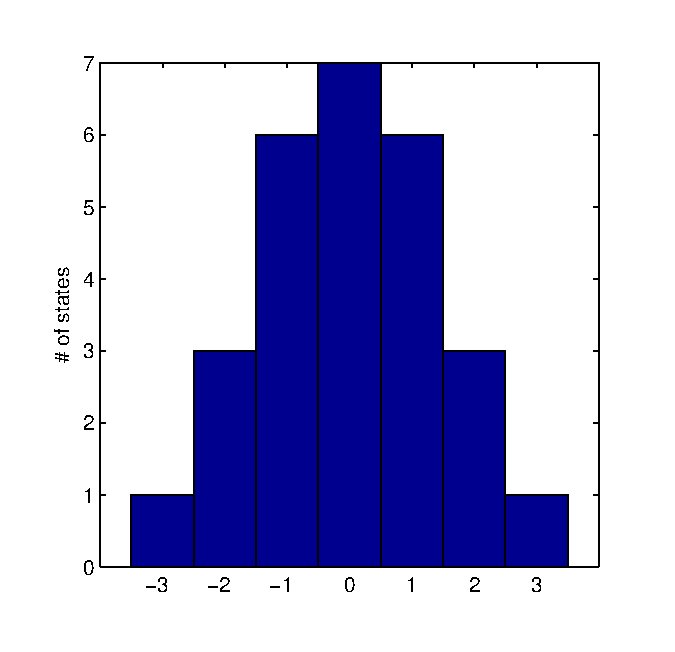
\includegraphics{p3}
\\
a) With all state having probability $\frac{1}{27}$ the entropy is 3.2958.\\
b) The entropy when only $M_z=0$ is possible is 1.9549. \\
c) The entropy when only $M_z=M$ is possible is 1.7918. \\
d) There is only one state with $M_z=3M$, so the entropy is 0.\\
e)


\section{Problem 4}
In class it was shown that $\frac{\partial U}{\partial \beta}=<(\Delta E)^2>$. 
To work out $<(\Delta E)^3>$ we find $\frac{\partial^2 U}{\partial \beta^2}$.
\begin{gather}
 d\beta=-\frac{1}{kT^2}dT\\
 \frac{\partial U}{\partial \beta}=\frac{\partial U}{\partial T}\frac{\partial T}{\partial \beta}
  =kT^2\frac{\partial U}{\partial T}=kT^2C_v\\
 \frac{\partial^2 U}{\partial \beta^2}=\frac{\partial}{\partial T}(\frac{\partial U}{\partial \beta})\frac{\partial T}{\partial \beta} \\
 \frac{\partial^2 U}{\partial \beta^2}=\left(2kTC_v+kT^2\frac{\partial C_v}{\partial T} \right)kT^2\\
 \frac{\partial^2 U}{\partial \beta^2}=k^2\left(2T^3C_v+T^4\frac{\partial C_v}{\partial T} \right)
\end{gather}
For an ideal gas $U=\frac{3}{2}NkT$ and $C_v=\frac{3}{2}Nk$. So we have:
\begin{gather}
 <(\Delta E)^2> = kT^2C_v=\frac{3}{2}Nk^2T^2\\
 <U^2>=(\frac{3}{2}NkT)^2\\
 <(\frac{\Delta E}{U})^2>=\frac{2}{3N}\\
 <(\Delta E)^3>=k^2(2T^3(\frac{3}{2}Nk)+T^4(0))=3Nk^3T^3\\
 <U^3>=\frac{3^3}{2^3}N^3k^3T^3\\
 <(\frac{\Delta E}{U})^3>=\frac{2^3}{3^3}\frac{1}{N^2}=\frac{8}{9N}
\end{gather}

\section{Problem 5}
For an ideal gas the entropy is $S=Nk\left(\ln{\frac{V}{N\lambda ^3}}+\frac{5}{2} \right)$.
We show that:
\begin{gather}
 \frac{S}{Nk}=\ln{(\frac{Q_1}{N})}+T(\frac{\partial \ln{Q_1}}{\partial T})_P
\end{gather}
The partition function for an ideal gas is $Q_n(V,T)=\frac{1}{N!}(\frac{V}{\lambda ^3})^N$.
$Q_1$ is $\frac{V}{\lambda ^3}$. We expand $Q_1$ and find $(\frac{\partial \ln{Q_1}}{\partial T})_P$.
\begin{gather}
 Q_1=\frac{V}{h^3}(2\pi mkT)^{3/2}\\
 (\frac{\partial \ln{Q_1}}{\partial T})_P=\frac{1}{Q_1}\frac{\partial Q_1}{\partial T}\\
 (\frac{\partial \ln{Q_1}}{\partial T})_P=\frac{3}{2}\frac{1}{T}
\end{gather}
We see that $\frac{S}{Nk}=\ln{(\frac{Q_1}{N})}+T(\frac{\partial \ln{Q_1}}{\partial T})_P=\ln{\frac{V}{N\lambda ^3}+\frac{3}{2}}$.


\end{document}
